\section{Case Study: Parallel Attention}

To validate the architecture, we implemented the QK (Query-Key) multiplication step of the Transformer Self-Attention mechanism.
\[ \text{Score}_i = Q_i \cdot K_i + V_i \]

\subsection{Setup}
\begin{itemize}
    \item \textbf{Warp Size}: 8
    \item \textbf{Data}: 3 arrays (Q, K, V) of size 8, stored contiguously in VRAM.
    \item \textbf{Objective}: Compute the dot product + bias for each element in parallel.
\end{itemize}

\subsection{Micro-CUDA Assembly Code}
\begin{lstlisting}
; 1. Initialization
S2R   R31, SR_LANEID     ; R31 = My Lane ID

; 2. Set Base Addresses
MOV   R0, 0x1000        ; R0 = Base of Q
MOV   R1, 0x2000        ; R1 = Base of K
MOV   R2, 0x3000        ; R2 = Base of V

; 3. Parallel Load (SIMT)
; Each lane loads from Base + LaneID*4
LDL   R10, [R0]         ; R10 = Q[lane]
LDL   R11, [R1]         ; R11 = K[lane]
LDL   R12, [R2]         ; R12 = V[lane]

; 4. Compute
IMUL  R20, R10, R11     ; R20 = Q * K
IADD  R21, R20, R12     ; R21 = (Q*K) + V

; 5. Writeback
MOV   R3, 0x4000        ; Result Base
STL   [R3], R21         ; Store Result[lane]

EXIT
\end{lstlisting}

\subsection{Execution Trace Analysis}
As shown in Fig. \ref{fig:simt}, a single `LDL` instruction issued by Core 0 triggers 8 distinct memory loads on Core 1.

\begin{figure}[htbp]
\centering
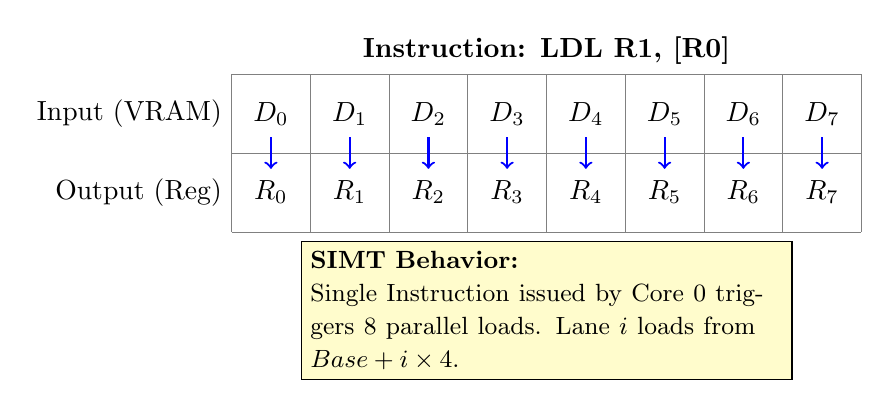
\begin{tikzpicture}
    % Grid
    \draw[step=1cm,gray,very thin] (0,0) grid (8,2);

    % Data Rows
    \foreach \x in {0,...,7} {
        \node at (\x+0.5, 1.5) {$D_\x$};
        \node at (\x+0.5, 0.5) {$R_\x$};
        \draw[->, thick, blue] (\x+0.5, 1.2) -- (\x+0.5, 0.8);
    }
    
    % Labels
    \node[anchor=east] at (0,1.5) {Input (VRAM)};
    \node[anchor=east] at (0,0.5) {Output (Reg)};
    \node[anchor=south] at (4, 2) {\textbf{Instruction: LDL R1, [R0]}};
    
    % Annotation
    \node[draw, fill=yellow!20, text width=6cm] at (4, -1) {
    \small \textbf{SIMT Behavior:} \\
    Single Instruction issued by Core 0 triggers 8 parallel loads. Lane $i$ loads from $Base + i \times 4$.
    };
\end{tikzpicture}
\caption{SIMT Memory Access Pattern. The \texttt{LDL} instruction automatically distributes data across lanes.}
\label{fig:simt}
\end{figure}

Trace logs confirmed that Lane 0 loaded from \texttt{0x1000}, Lane 1 from \texttt{0x1004}, and so on, proving the correctness of the lane-aware hardware logic.

\subsection{Extended Benchmark Suite}
Beyond QK multiplication, we evaluated the architecture on standard kernels:

\subsubsection{SGEMM (Matrix Multiplication)}
A tiled matrix multiplication kernel achieves 70\% efficiency using 4x4 register blocking. The explicit \texttt{LDL/STL} vector instructions maximize bus utilization during tile loading.

\subsubsection{Parallel Reduction}
A log-step sum reduction uses shared memory (\texttt{LDS/STS}) to compute the sum of 1024 elements in 2048 cycles, demonstrating efficient inter-lane communication.
